\chapter{Approach}
\label{approach}
% Min: overly repetitive.  I have read similar sentences at least a few times already.  Excise the excess mentions.  DRY.
We describe how we adopt a supervised learning approach to tackle the problem that we had decomposed into two tiers.

\begin{figure}[h]
  \centering
  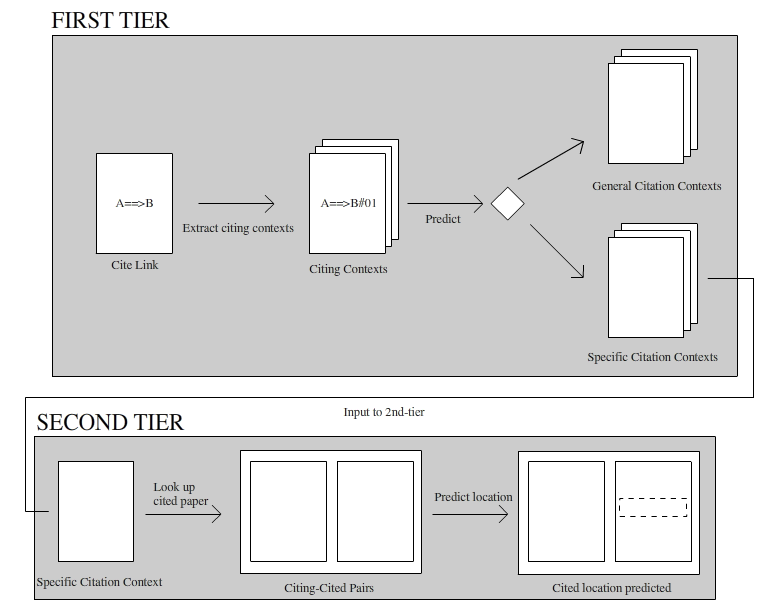
\includegraphics[scale=0.60]{./twotier}
  \caption{A Two-Tier Approach}
  \label{fig:twotier}
\end{figure}

\section{{\it GvS} (First Tier)}
\label{firsttier}
{\it GvS}, short for General versus Specific, is the first tier in our approach. In {\it GvS}, we perform a binary \textit{citation classification} task, which is already a challenging task. 
% Min: I don't see the point of this sentence
%We are not interested in determining whether the citation is one of the 12 class as defined by \cite{teufel2009annotation}, but only whether it is General or Specific. 
{\it GvS} makes use of information only from the citing contexts in a citing paper. We built a model based on features extracted from the citing contexts. With this model, {\it GvS} classifies citing contexts into one of the two classes. 
% Min: repeated again??
%Only those contexts that are classified as Specific will be passed to the second tier.

\subsection*{Building The Model For {\it GvS}}
% Min: GLOBAL: replace Table \ref => Table~\ref.  Same with other references to Figures, etc.
% Min: You need to say why you adopted these features and whether you added any new features.
{\it GvS} performs citation classification. Thus to build our model, we adopt past features used in \outcite{dongensemble} previously used for citation classification. In addition, based on the observations made during annotation, we introduced a few features that are targeted at Specific citations. From each of the 275 annotated cite links mentioned in Table~\ref{tab:annotation} we extracted a set of features into a {\it feature vector} and map it to its {\it label} according to annotation (Figure~\ref{fig:featurevector}). The features used are as described below. Note that the features with names beginning with the asterisk (*) are new features we introduced.

\begin{figure}[h]
\centering
$v_1:[f_1, f_2, f_3, \ldots, f_n] \rightarrow L_1$ \\
$v_2:[f_1, f_2, f_3, \ldots, f_n] \rightarrow L_2$ \\
$\vdots$ \\
$v_i:[f_1, f_2, f_3, \ldots, f_n] \rightarrow L_i$ \\
$\vdots$ \\
$v_m:[f_1, f_2, f_3, \ldots, f_n] \rightarrow L_m$
\caption{Mapping feature vectors to labels from annotation}
\label{fig:featurevector}
\end{figure}

\subsection*{{\it GvS} Features}
\begin{enumerate}
\item Physical Features (Feature $A$)\\
We adopted wholesale the physical feature set as presented in \cite{dongensemble}. They are:
\begin{enumerate}
\item \textit{Location}: in which section the citing sentence is from.
\item \textit{Popularity}: number of citation marks in the citing sentence.
\item \textit{Density}: number of unique citation marks in the citing sentence and its neighbour sentences.
\item \textit{AvgDens}: the average of Density among the citing and neighbour sentences.
\end{enumerate}

% Min: this only gives the reasoning for a particular feature.  What about the other three?
The intuition for using these features is that: Based on our observations, citations found in the Evaluation section of the citing paper tend to cite results from the Evaluation section of the cited paper. Thus the \textit{location} would suggest the type of citation. Also, General citations tend to have a higher number of citation marks within a citing sentence and its neighbour sentences. This is the rationale for the remaining 3 features.

%% Min: make sure that you mark these features as new that you invented.  I've tried to add.
%Based on the previously-described analysis in Chapter~\ref{buildingcorpus}, we also designed and implemented four new features, for the first Tier task: 

\item *Number Density (Feature $B$)\\
A numeric feature similar to the first feature set that measures the density of numerical figures in the citing context. This is based on our previously-described analysis in Chapter~\ref{buildingcorpus} that Specific citations tend to refer numerical figures in evaluation results in the cited paper. E.g. ``...Nivre and Scholz (2004) obtained a precision of 79.1\%...".

\item *Published Year Difference (Feature $C$)\\
A numeric feature that represents difference in the publishing year between the citing and cited paper. A large difference means that a large publishing time gap exists between the citing and cited papers.  Such long term citations are usually citations for General purposes.

\item *Citing Context's Average \url{tf-idf} Weight (Feature $D$)\\
A numeric feature that indicates the average number of \textit{valuable} words, as determined by TF$\times$IDF \cite{irtextbook} in the citing context. Higher values suggest important, signature words pertinent to a specific claim.  Thus high values of this feature we believe indicate a Specific use.

\item Cue Words (Feature $E$)\\
Another numeric feature adapted from \outcite{dongensemble} that computes the count of specific cue words that appear in the citing sentence and its neighbouring sentences. We defined two classes of cue words: Cue-General and Cue-Specific (refer to Appendix~\ref{cuewords} for list of cue words). These cue words were hand-picked, based on examples observed during the annotation process.
\end{enumerate}

Recall that according to our annotation statistics, this task is heavily skewed towards General citations. Building a model based on this skewed set of data instances will produce a biased model that often predicts General. In fact, during some preliminary experiments where all data instances are fitted into the model, it outputs General for all its predictions. To address this problem, we train the model on artificially sampled {\it unskewed data}.  From the set of labelled feature vectors, we first gathered the Specific instances. Then we {\bf randomly} selected from the rest to have a $1:1$ of Specific vs. General instances. While this ratio appear unrealistic compared to the actual statistics, we argue that we are building a model using balanced data to measure its ability to differentiate between the two types of citation.

\section{{\it LocateProv} (Second Tier)}
\label{secondtier}
{\it LocateProv}, short for Locate Provenance, is the second tier of my approach. The design of {\it LocateProv} is all its inputs are Specific citations predicts which of the fragments in the cited paper is the cited fragment. Resembling a search, in {\it LocateProv} the citing context becomes the {\it query} to match the cited fragments in the cited paper. To perform this ranking task, we import features that are prevalent that are basic mechanisms for ranking in Information Retrieval.

\subsection*{Building The Model For {\it LocateProv}}
In {\it LocateProv}, we predict which cited fragment is the provenance of a citation. Instead of cite links, we used the annotated fragments in Table~\ref{tab:annotation} to build the model. Unlike the first tier, the features used in the second tier are based on both the citing contexts and the cited fragments. Similarly the feature vectors are mapped onto the annotated labels. Adopting the same notation as used in the first tier, in the list of features below, features with names beginning with an asterisk (*) are features we introduced.

\subsection*{{\it LocateProv} Features}
\begin{enumerate}
\item *Surface Matching (Feature $F$)\\
A numeric feature that measures the amount of word overlap between the citing sentence and a fragment in the cited paper.

\item *Number Near-Miss (Feature $G$)\\
A numeric feature that measures the amount of numeric figures overlap between the citing sentence and a fragment in the cited paper. This feature will preprocess each fragment, rounding numbers or converting to percentage values when it tries to match similar numbers in the citing sentence. This feature was added because of the observations we made earlier in Chapter \ref{buildingcorpus}, that citations may refer to evaluation results in the cited paper.

\item *Bigram Matching (Feature $H$)\\
% Min2: is this a percentage or an absolute number?
A numeric feature that measures the percentage of bigrams overlap between the citing sentence and a fragment in the cited paper. This feature was added to preserve word order when comparing the citing sentence and the fragment. This feature was also targeted at Specific citations that refer to term definitions or quote directly.

\item Cosine Similarity (Feature $I$)\\
% Min2: give formula
\begin{equation}
\textrm{cosine similarity} = \frac{v \cdot u}{|v| |u|}
\end{equation}
A feature commonly used in information retrieval to measure similarity between the query and a candidate document. In our case, citing sentence and the fragment. $v$ is a vector representation of the citing sentence and $u$ is the fragment.
\end{enumerate}
Most of these features are added based on some of the observations we made during the annotation tasks.

Recall that the data instances that were annotated are heavily skewed against Specific citations. In fact, the ratio of Specific-Yes instances compared to the rest is at least $1:1000$. It is impossible to train a model that is not biased with this entire set of instances. Hence we used the same method used in {\it GvS}: to use a $1:1$ of Specific-Yes vs Specific-No instances. Note that this also coincide with the design of {\it LocateProv} that inputs are only Specific citations. It was also not feasible to use the actual ratio between Specific-Yes and Specific-No because comparing a citing-cited pair of papers, the ratio of citing context to the number of fragments in the cited paper is easily $1:100$.

For both tiers, we trained the models using various classifiers and evaluated their performance. We discuss the evaluation process in the following chapter.
